\documentclass[a4paper,10pt]{article}
\usepackage{fancyvrb}
\input{/Users/benjamin/Documents/Education/LaTeX/macro.tex}

\title{AEV: S�ance 2}
\author{Benjamin \bsc{Van Ryseghem}}

\begin{document}
\maketitle

\section{Exercice 1}
\begin{Verbatim}[commandchars=\\\{\}]
entity exo1 is
port( clk: in bit;
a: \emph{in} bit_vector (\emph{4} downto 0),
s: out bit_vector (\emph{2} downto 0);
end exo1;

architecture aexo1 of exo1 is
begin
with \emph{a} select
s <= \emph{"101"} when "01001",
	"011" when "10010",
	\emph{"001"} when others;
end aexo1;


\end{Verbatim}

\section{Exercice 2}
\begin{itemize}
	\item [] \verb?<=? affectation de signaux
	\item [] \verb?:=? affectation direct
	\item [] \verb?=? comparaison
\end{itemize}
\subsection{Question 1}
\begin{tabular}{|c|c|c|}
\hline
a & b & s \\
\hline 
\hline
0 & 0 & 1 \\
0 & 1 & 0 \\
1 & 0 & 0 \\
1 & 1 & 1 \\
\hline
\end{tabular}

Cela �quivaut � un "not xor".

\subsection{Question 2}
\cf Figure~\ref{ex2}.


\begin{figure}[ht]
\begin{center}
     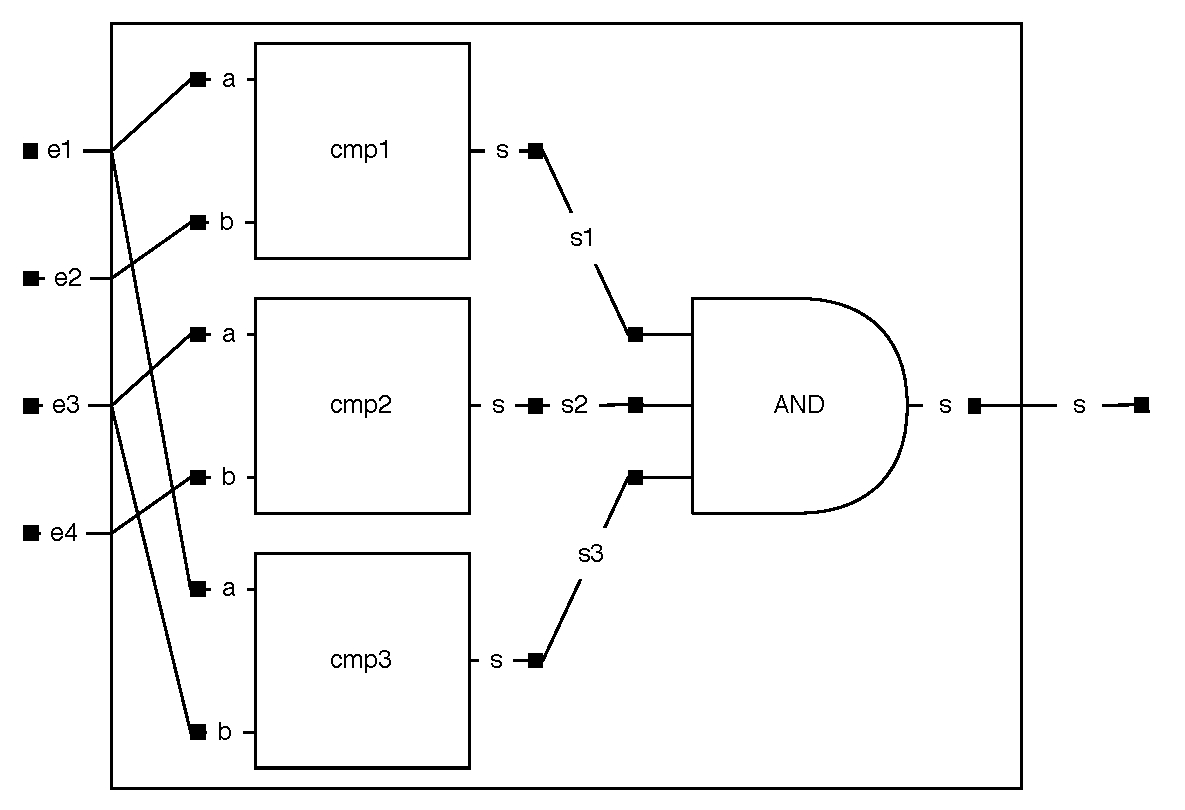
\includegraphics[width=15cm]{figures/ex2}
\end{center}
     \caption{Analyse structurelle}
     \label{ex2}
\end{figure}

\subsection{Question 3}
Ce circuit est un \emph{comparateur 4 bits}.

\section{Exercice 3}
\subsection{Question 1}
\begin{verbatim}
entity circuit is 
       port (A, B, Cin : in std_logic;
               S, Cout : out std_logic);
end circuit;

architecture archi_circuit of circuit is
       s <= A Xor B Xor Cin;
       Cout <= (A AND B) OR (A XOR B) AND CIN;
\end{verbatim}

\signature

\end{document}